\chapter{Experiments}
The main goal of this work was to use proximal policy optimization to simulate a parking situation in a virtual environment.

The tool used to create the simulation was Unity (version 2021.3.7f1), developed by Unity Technologies, commonly used as a game engine. All the assets used are available for free in the Unity Store.

Unity provides a open-source \textit{toolkit} called ML-Agents, which enables developers to create and train AI agents inside the platform. ML-Agents also provides its own implementation of proximal policy optimization, as described in \cite{schulman2017proximal}.

The first experiment is the simplest, where we keep every spawn fixed across all episodes. In the following experiments, we randomize the spawns of the agent, parking spot and obstacles (parked cars), until the environment is completely random.
\section{Experiment 1: Fixed Positions}
We design a fairly simple parking scenario with a few cars already parked serving as obstacles.
\begin{figure}
    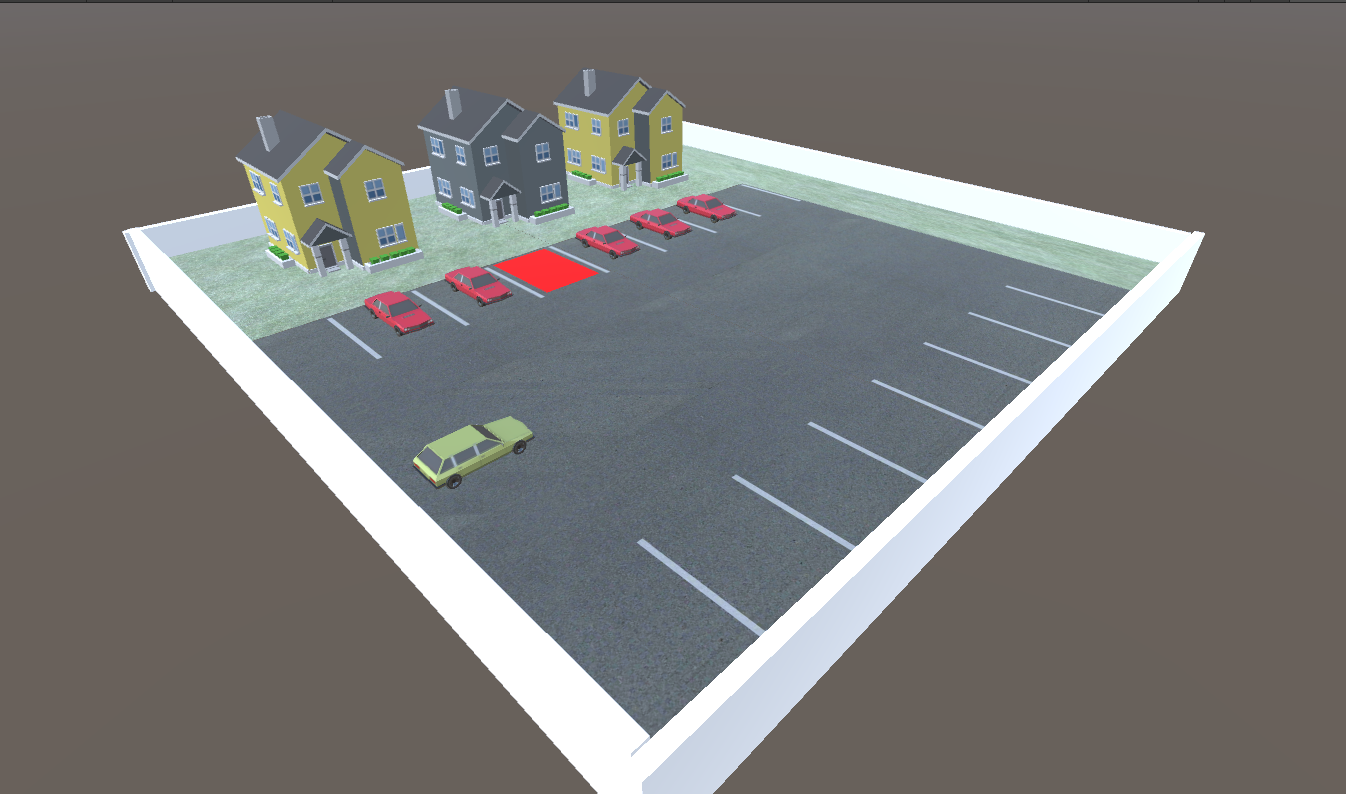
\includegraphics[width=\textwidth]{environment}
    \caption{The parking lot environment in Unity Engine}
\end{figure}
The environment is a one floor parking scenario with a total of 16 parking spots. For this first experiment, the designated parking spot is fixed, as well as the other cars' positions. The car is considered to be parked when it stays within $0.6$ units from the spot for at least $0.5$ seconds. A unit in Unity is equivalent to 1 meter and the distance is computed from the center of the car to the center of the parking spot.

The agent is a low-polygon 3D car model equipped with a total of 24 depth sensors which can detect objects up to 5 units away.
\begin{figure}[H]
    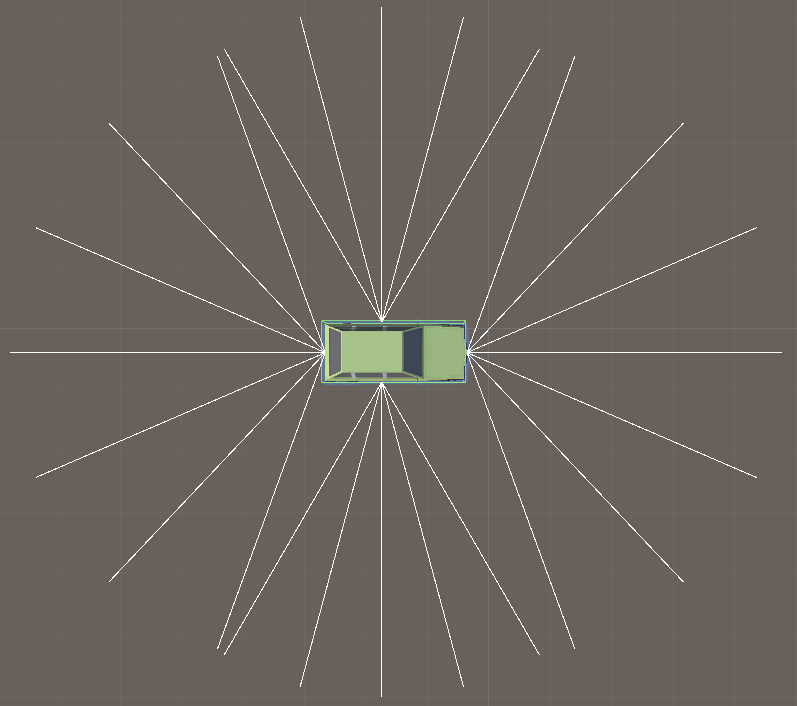
\includegraphics[width=\textwidth]{car}
    \caption{The car (agent) and its sensors}
\end{figure}
The reward functions are described in the table below:
\begin{table}[H]
\begin{tabular}{|l|c|}
\hline \multicolumn{1}{|c|}{ Reward function } & Value \\
\hline Timeout & $-1000$ \\
\hline Parking successfully & $1000$ \\
\hline Parking successfully and sufficiently aligned & $5000$ \\
\hline Time & $-0.0002$ per timestep \\
\hline Stopping & $-0.0002$ per timestep \\
\hline Collision & $-1$ \\
\hline Stay in collision & $-0.5$ per timestep \\
\hline Goal heading & $-1$ to $1$ per timestep, see below for details\\
\hline Goal distance & $-1$ to $1$ per timestep, see below for details\\
\hline
\end{tabular}
\end{table}
During the first few experimental runs, we tried multiple ways of encouraging the agent to get closer to the goal, but, of course, without actually telling the exact coordinates. Rewarding it for getting closer compared to the previous time step was our first successful attempt at teaching the agent to park at the designated spot, but the success rate was still rather low. The agent would often get stuck in a loop going back and forth and the episode would eventually end due to timeout.

With the intent of proving a better incentive for getting closer, we designed a custom curve to define the rewards the agent would get based on its distance from the parking spot.
\begin{figure}[H]
    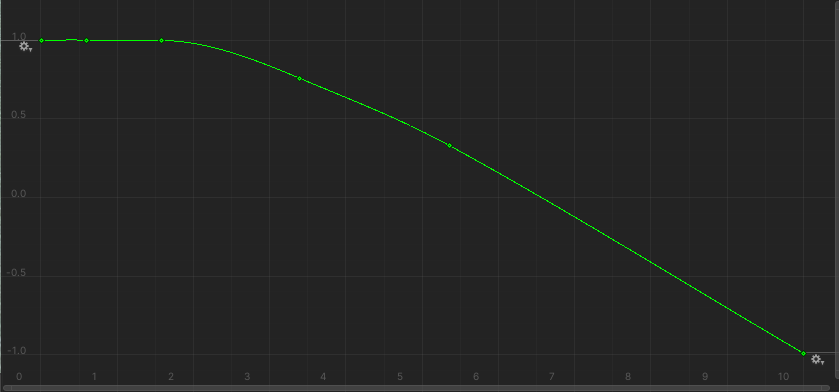
\includegraphics[width=\textwidth]{goal_reward_curve}
    \caption{The reward function for getting closer to the goal}
    \label{fig:goaldist}
\end{figure}
The $x$-axis ranges from $0$ to $10$ and represents the distance between the agent and the goal. The $y$-axis ranges from $-1$ to $1$ and increases as the agent gets closer to the spot. From the very first attempt, these reward functions showed very good results, with success rates above $50\%$. However, the agent would often park completely disaligned.

To seek further improvement, we also rewarded the agent at each time step for heading towards the goal (note that this is invariant of distance). The reward is the dot product between the vector pointing forward from the car and the vector pointing forward from the parking spot, such that the reward is $1$ when the agent and the parking spot are perfectly aligned and $-1$ when the agent is headed the complete opposite way. Adding this extra reward function not only increased the success rate to almost $100\%$, but also significantly decreased training time. Unfortunately, it hadn't solved the original issue.

As an second attempt, we added an extra criterion to define whether the agent is parked or not. If the dot product between the two vectors mentioned above is $\geq 0.9$ at the moment of parking, the reward of $1000$ is given and the episode ends. If the dot product is $\geq 0.97$ the reward is increased to $5000$. In terms of angles, since both vectors are unitary, the dot product is simply the cosine between the two vectors, that is, the angle must be at most $45\degree$ to consider the agent parked and at most $\approx 25\degree$ to receive the bonus reward. In terms of training time and success rate, nothing has changed, but the agent would always park correctly and get the bonus.
\section{Experiment 2: Randomized Positions}
\subsection{Randomized Car Position and Fixed Parking Spot}
\subsection{Randomized Car and Parking Spot Positions}
\section{Experiment 3: Parallel Parking}